\chapter{Experimental Setup}
\label{chap:setup}

Knowledge about the components and techniques required for optimizing order placement was provided in Chapter \ref{chap:preliminaries}, and previous approaches were introduced in Chapter \ref{chap:related-work}.
The process of collecting historical event data and the construction of a limit order book was explained in Chapter \ref{chap:data}.
The data was investigated and theories were stated as a guideline for a future learning process.
However, in order to apply reinforcement learning, an environment has to be developed which is flexible enough to allow investigation regarding different types of features and learning algorithms that are incorporated in an agent.
The correctness of such an environment is critical as it emulates a stock exchange and therefore determines how orders would have been transacted in the past.
If the implementation varies from the one used in exchanges, or does not cover certain edge cases, the matching of placed orders would differ significantly from the one in a production setup.

This chapter aims to build an environment that emulates a subset of the capabilities of a real world exchange in order to determine how limit orders would have been processed, had they been placed at a given point in time in the past.
Therefore, the setup of the environment is described at first and explains how the required components work in combination such that a learner can simulate order placement.
Additionally, an extension of this environment is provided
to simulate simultaneous order placement on both sides of the book.
This process is commonly referred to as \textit{market making}.
Subsequently, feature engineering is described which incorporates previously stated theories and results in features that can be used by the agents.
Finally, two implementations of reinforcement learning agents are provided.
A Q-Learning agent will serve as the learner when no market variables are provided and a Deep Q-Network agent is developed to handle complex features.


\section{Order Placement Environment}
\label{sec:setup-order-placement}

The reinforcement learning environment (see Section \ref{sec:rl-environment}) that emulates order placement on historical market data is introduced in this section.
Thus, the environment enables an agent to buy or sell $V$ shares within a time horizon $H$.
Therefore, the previously described components (introduced in Chapter \ref{chap:preliminaries}) come into play.
The main idea of its working is that, the agent observes a state $s_t$ (so-called observation state) at some time $t$ and responds with an action $a_t$ that indicates at which price to place the order in the order book.
The task of the environment is then to evaluate the outcome of the placed order and report to the agent accordingly with a reward $r_{t+1}$ and the next state $s_{t+1}$.
Subsequently, the order is cancelled such that the agent can submit a new action for the remaining shares to be bought.

OpenAI Gym \cite{brockman2016openai} is an open source toolkit for reinforcement learning.
The interfaces of this toolkit were used in order to follow their standards while building this environment.
The advantage of which is that any OpenAI Gym compatible agent and bench-marking tools can make use of this environment.

\subsection{Overview of components}

\begin{figure}[H]
    \centering
    \makebox[\linewidth]{
        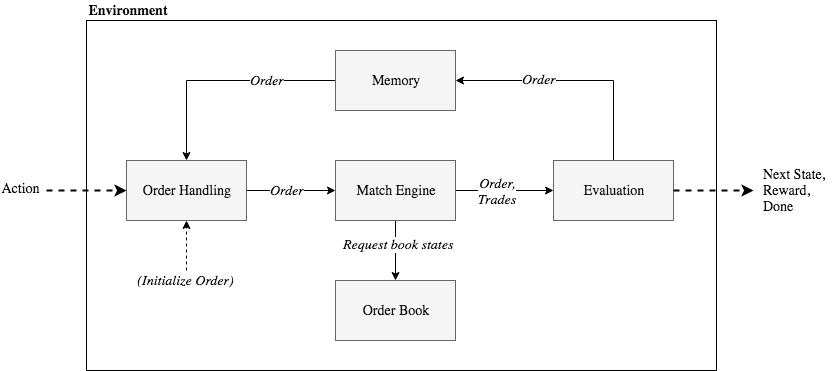
\includegraphics[width=14cm]{images/rl-env-overview}
    }
    \caption{Overview of reinforcement learning order placement environment.}
    \label{fig:rl-env-overview}
\end{figure}

Figure \ref{fig:rl-env-overview} shows the inner workings of the order placement environment.
The process is initialized and driven by an agent sending an action to the environment.
The first component to react upon receiving the action is the \textit{order handling component}, which determines whether the agent is currently trying to fill an order, that is when the agent has started an epoch, or a new order needs to be created, that is when the agent starts an epoch.
In either case, the order price will be adjusted according to the received action.
Subsequently, the order is forwarded to the \textit{match engine}, which tries to execute the order within the historical data set that is represented by the \textit{order book}.
The order and the possible resulted trades evolved during the matching process are then forwarded to the \textit{evaluation component}.
Since it can take multiple steps for the agent to fill an order, the environment is required to have an internal state.
Therefore, the remaining inventory and the consumed time of the order is updated and stored in the \textit{memory}.
Additionally, the index of the last visited order book state is stored such that in a next step the match engine will proceed the matching where it stopped last.
In case no trades resulted during the matching process, only the consumed time is subtracted from the order.
Otherwise, the sum of the size of the trades is subtracted from the order's inventory.
Subsequently, the evaluation component calculates the reward based on the previously resulted trades.
Finally, the reward, the next observation state and whether or not the order is completely filled (e.g. the epoch is done) is finally forwarded to the agent.

\subsection{Configuration parameters}

For the environment to be flexible, such that agents can place orders in various settings, configuration parameter have to be defined.
The \textit{order side} $OS$ (previously defined in Eq. \ref{eq:order-side}) specifies whether the orders, which are created within the environment, are intended to be buy or sell orders.

\begin{figure}[H]
    \centering
    \makebox[\linewidth]{
        
\includegraphics[width=10cm]{images/setup-time-horizon}
    }
    \caption{Segmented time horizon $H$ with remaining time $t$.}
    \label{fig:setup-time-horizon}
\end{figure}

The time horizon $H$ defines the amount of time given in order fill an order.
The default time horizon is 100 seconds for reasons described in Section \ref{sec:execution-definition}, which reflects the Good-Till-Time (see \ref{sec:ob-characteristics}) of the order.
As illustrated in Figure \ref{fig:setup-time-horizon}, the time horizon is segmented into discrete time steps $t$ and therefore limits the number of steps an agent can take within one epoch.
Each step is of the same length $\Delta{t}$, which is for illustration purposes set to 10 seconds.
We pick $T$ as the maximum value of $t$, indicating that the entire amount of time is remaining, whereas $t=0$ states that the time horizon is consumed.
Consequently, within an epoch the GTT of the order is being adjusted to $\Delta{t}$ for each step, still resulting in a total GTT of $H$.
Therefore, if the order is not completely filled after the last step was taken, a market order follows in order to get to the final state.

Lastly, a \textit{feature type} has to be defined which determines the state observed by the agent.

\subsection{State}
Unlike in most traditional reinforcement learning environments, each step taken by the agent leads to a complete change of the state space.
Consider a chess board environment, where the state space is the board equipped with figures. 
After every move taken by the agent, the state space would look exactly the same, except of the figures moved with that step.
The epoch would continue until the agent either wins or looses the game and the state space would be reset to the very same setup for each epoch.
In the order placement environment however, it is, as if, for each step not only one or two figures of the chess board change their position, but almost all of them.
And a reset of the environment will result in an ever changing setup of the figures on the chessboard.
The reason for this is that the chessboard is in our case the order book that underlies a time series which evolves over time.
More precisely, the state space $S$ is defined as a sequence of order book states, from which an agent can observe an observation state $O$.
Important to note is the criteria for reaching the final state; that is, when the entire inventory was bought or sold--Checkmate!.

There are two general types of variables that can be used in order to create an observation state: \textit{private variables} and \textit{market variables}.

\begin{figure}[H]
    \centering
    \makebox[\linewidth]{
        
\includegraphics[width=10cm]{images/setup-inventory}
    }
    \caption{Inventory of $V$ segmented shares with a remaining inventory $i$.}
    \label{fig:setup-inventory}
\end{figure}

For private variables, the size of the state space depends on the $V$ shares that have to be bought or sold and the given time horizon $H$, resulting in a state $s \in R^2$.
However, fractions of shares and time which evolve during the matching process would result in a vastly large state space.
Therefore, similar to the discrete time steps which are described above, the $V$ shares are divided into discrete inventory units $i$ of size $\Delta{i}$, as illustrated in Figure \ref{fig:setup-inventory}.
The inventory units approximate the order size in order for our policy to distinguish between when creating an order.
We pick $I$ as the maximum value of $i$, indicating that the entire inventory remains to be filled.
The order is considered as filled when $i=0$, meaning that no inventory is left.
Given the inventory units and the time steps, the state space remains $s \in R^2$ but becomes much smaller in its size, namely $I \times H$.
In the default setup a segmentation of 0.01 BTC steps is applied.
For example, if the initial inventory is 1.0 BTC and the order is partially filled with 0.015 BTC during an epoch, the remaining inventory is 0.99 BTC (instead of 0.985) for the next step the agent will take.

Market variables can be any information derived from the order book at a given moment in time.
Therefore the specified feature set (see Section \ref{sec:feature-engineering} below), results in some state $s \in R^d$, whereas $d$ is the dimension of the feature set.
Consequently, market variables increase the state space drastically, due to (1) the initialization of the environment using a random order book state and (2) the dimensionality of the feature set.
Hence, for each step taken by the agent, the order book states are likely to be different and thus the state the agent observes changes equally. 

\subsection{Action}

A discrete action space $A$ is a vector $(a_{min}, . . . , a_{max})$ that represents a range of relative limit levels an agent can choose from in order to place an order. 
That is, how deep ($a_{min}$) and how high ($a_{max}$) the order can be placed in the book.
The action $a \in A$ is an offset relative to the market price $p_{m^T}$ before the order was placed (at time step $t=T$).
Negative limit levels indicate the listing deep in the book and positive listings relate to the level in the opposing side of the book.
Hence, the price of the order placement $p$ at some time step $t$ is $p_t = p_{m^T} + a_i * \Delta{a}$, whereas $\Delta{a}$ is the step size of an action.
An illustration of this concept is given in Figure \ref{fig:setup-actions}.
\begin{figure}[H]
    \centering
    \makebox[\linewidth]{
        
\includegraphics[width=8cm]{images/setup-actions}
    }
    \caption{Actions represent an offset relative to the order price at which to place the order in some order book state $OS_i$ at some time step $t$.}
    \label{fig:setup-actions}
\end{figure}

By default the action step size $\Delta{a}=\$0.10$.
For example, with $|A|=5$ that is $(p_{m^T}-0.2, p_{m^T}-0.1, p_{m^T}, p_{m^T}+0.1, p_{m^T}+0.2)$.
The action space is configurable and the default implementation is of size $|A|=101$, indicating that $a_{min}=-50$ and $a_{max=50}$ result in an order price $p=p_{m^T}-\$5$ and $p=p_{m^T}+\$5$ respectively.

\subsection{Reward}

The reward is defined as the difference of the market price before the order was placed $p_{m^T}$ and the volume weighted average price (Eq. \ref{eq:vwap}) paid or received after the order has been filled. 
Hence, for buying assets the reward is defined as $r=p_{m^T}-p_{vwap}$ and for selling assets $r=p_{vwap}-p_{m^T}$.
In case no trades resulted during the matching process, the reward is $r=0$, indicating that no direct negative reward is provided.
Reasons for this are that in case the order could not be matched over the course of the time horizon, a market order which likely produces trades with a worse price than the market price before the placement has started.
Given the definition of the discounted return (Eq. \ref{eq:discounted-return}) we calculate $R_t=\sum_{t'=t}^{t_0}{\gamma^{t'-t}*r_{t'}}$, where $t_0$ is the time step at which the agent has its time horizon for the ongoing order fully consumed.

\section{Market making Environment}

TODO

\section{Feature engineering}
\label{sec:feature-engineering}



\section{Q-Learning agent}

One of the reinforcement learning algorithms used in this work is known as \textit{Q-Learning}. 
The name derives from the application of the previously presented Q-function (Eq. \ref{eq:q-function}), more specifically its use within the Bellman equation (\ref{eq:bellman}) that undergoes an iterative update.
\\
\\
The general idea is ... 

\section{Deep Q-Network agent}
